% == == == == == == == == == == == == == == == ==
%
%   A sample latex file for UoY, Dept. Electronics
%   Lab reports. This is NOT an official document
%   Just some thing I find useful when starting a
%   lab report in latex.
%
%   By  Zak R. A. West, zraw500@york.ac.uk
%
%   Licensed under the GNU GPL v2.0 license
%
% == == == == == == == == == == == == == == == ==

% Use the article class with font size 11pt
\documentclass[12pt]{article}

% Creates placeholder text (Only needed for this example)
\usepackage{blindtext}

% Deal with language and encoding
\usepackage[T1]{fontenc}
\usepackage[utf8]{inputenc}
\usepackage[english]{babel}

% setup page size
\usepackage{geometry}
\geometry{a4paper,margin=2in,lmargin=1in,rmargin=1in} % reduced margins

% Set up fancy headers and footers
\usepackage{fancyhdr} 
\pagestyle{fancy} % options: empty , plain , fancy
\renewcommand{\headrulewidth}{1pt} % adds line at the bottom of the header

% Set up table of contents
\usepackage[nottoc,notlof,notlot]{tocbibind}
\usepackage[titles,subfigure]{tocloft}

% Set up graphics and figures
\usepackage{graphicx}
\usepackage{wrapfig}
\usepackage{subfig}

% Better tables in latex
\usepackage[table,xcdraw]{xcolor}
\usepackage{booktabs} 
\usepackage{multirow}

% Begin paragraphs with an empty line rather than an indent
\usepackage[parfill]{parskip}

% For including code 
%\usepackage{verbatim}
\usepackage{listings}
\usepackage{color}

% Setup colors for code highlighting
\definecolor{commentcolor}{rgb}{0,0.4,0}
\definecolor{stringcolor}{rgb}{0.5,0.8,0.5}
\definecolor{identifiercolor}{rgb}{0.1,0.1,0.1}
\definecolor{keywordcolor}{rgb}{0.2,0,0.9}

\definecolor{numbercolor}{rgb}{0.5,0.5,0.5}
\definecolor{backgroundcolor}{rgb}{0.975,0.975,0.975}

% Setup style of code listings
\lstset{
  breakatwhitespace=false,
  breaklines=true,
  commentstyle=\itshape\color{commentcolor},
  frame=leftline,
  backgroundcolor=\color{backgroundcolor},
  keepspaces=true,
  keywordstyle=\bfseries\color{keywordcolor},
  identifierstyle=\color{identifiercolor},
  numbers=left,
  numbersep=10pt,
  numberstyle=\small\color{numbercolor},
  rulecolor=\color{black},
  showspaces=false,
  showstringspaces=false,
  showtabs=false,
  stepnumber=1,
  stringstyle=\color{stringcolor},
  tabsize=2,
  title=\lstname
}

% Better maths rendering
\usepackage{array}

% For more list types
\usepackage{paralist}

% Better section formatting
\usepackage{sectsty}

% Sets up formatting for section headings
\allsectionsfont{\sffamily\mdseries\upshape}
\renewcommand{\cftsecfont}{\rmfamily\mdseries\upshape}
\renewcommand{\cftsecpagefont}{\rmfamily\mdseries\upshape}

% Set up header and footer text
\makeatletter
\lhead{\@title}\chead{}\rhead{\@author}
\lfoot{}\cfoot{\thepage}\rfoot{}
\makeatother

% Should show blue underlines on links, but it doesn't appear to work
\usepackage[colorlinks=false, allbordercolors={0 0 0}, linkbordercolor=blue, pdfborderstyle={/S/U/W 1}]{hyperref}

% Tell latex that your images are in a folder called Images
\graphicspath{{Images/}}

% Use url for better url handling
\usepackage{url}

% Use biblatex for citations
\usepackage{csquotes}
\usepackage[
  backend=biber,
  style=numeric,
  sorting=ynt
]{biblatex}
\addbibresource{references.bib}

% My custom title page package
\usepackage{UoYTitlePage}


%%% =====================================================
%%% =====================================================
%%%     You Should Only Have To Edit Stuff Below
%%%     Here. Unless You Want To Change The Style.
%%% =====================================================
%%% =====================================================


% ====================================
% Set up tile, author and other stuff
% ====================================

\uni{University of York}
\dept{Department of Electronics}

\module{Computer Architectures}
\project{Homework Two}

\title{Homework Two}
\author{Y3839090}

\supervisor{ }
\logo{logo}

\abstracttext{
	. . . 
}

% ====================================
% Start of the main document
% ====================================
\begin{document}

  % ============
  % Title Page
  % ============
  \maketitle

  % ============
  % Contents Page
  % ============
  \pagenumbering{roman} % Use roman numerals for page numbers
  \tableofcontents % Adds a table of contents
  \listoffigures % Adds a list of figures
  \newpage
  \pagenumbering{arabic} % Use Arabic (integer) numbering

  % ============
  % Main Pages
  % ============
  \section{Question 1}
    A Flowchart of the algorithm for paged segmentation, assuming the presence of separate translation look aside buffers (TLBs) for pages and segments.
    \begin{figure}[ht]
      \centering
      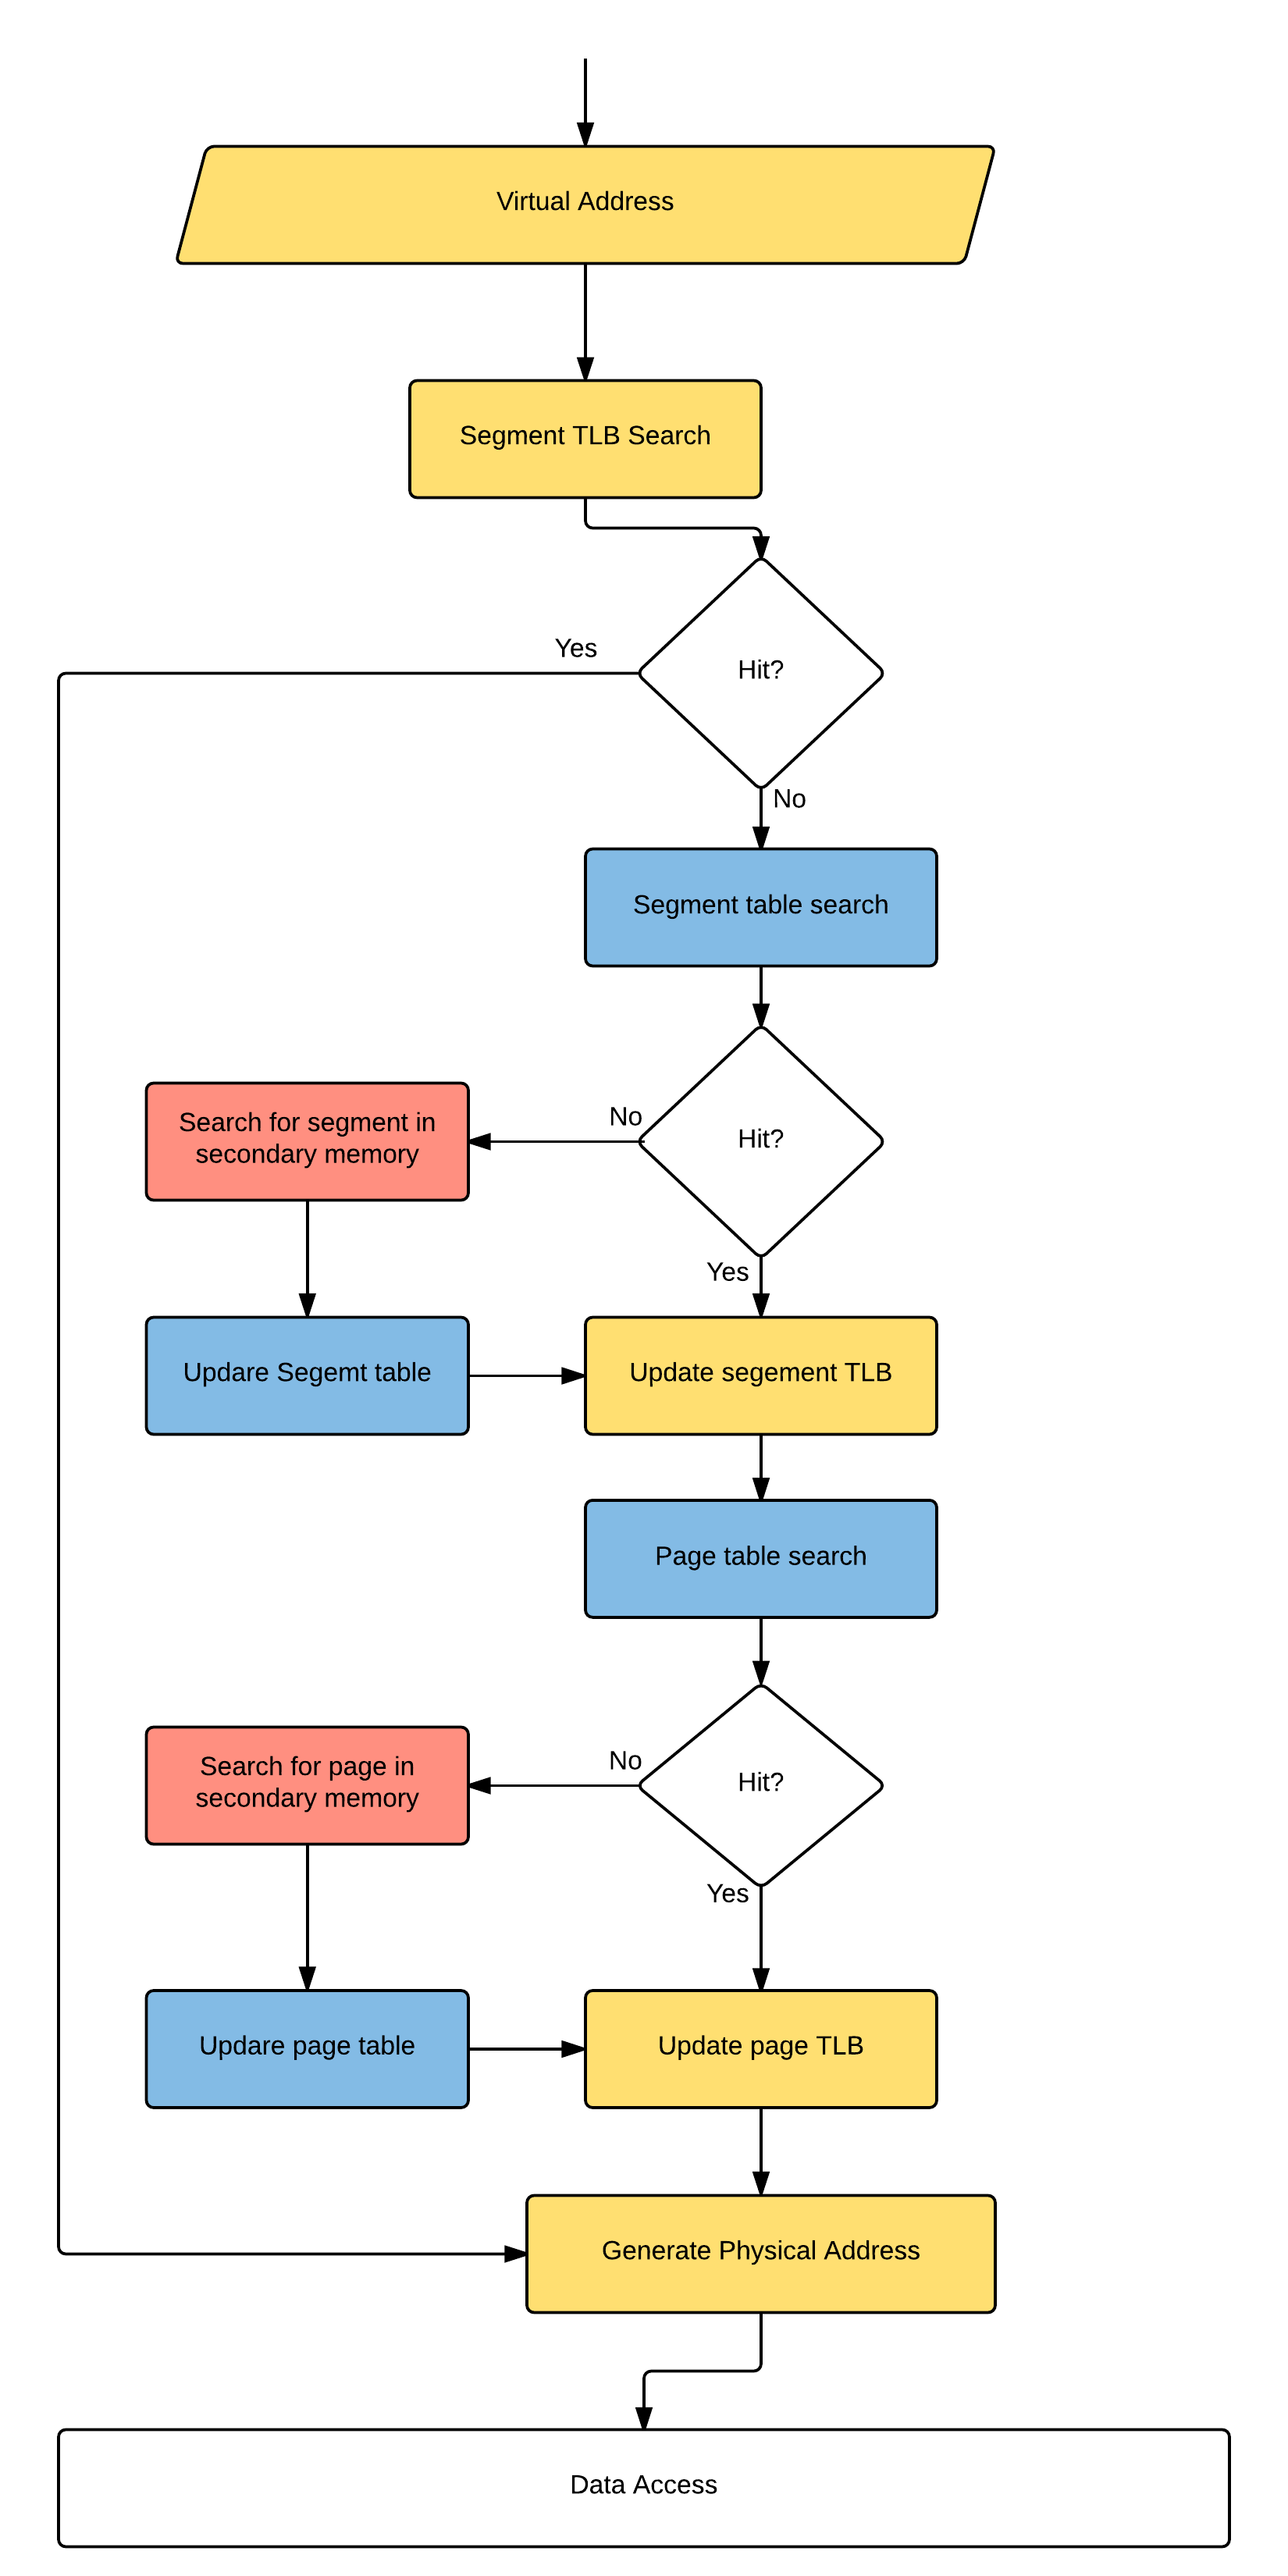
\includegraphics[height=1\textwidth]{Paged_Segmentation_Flowchart.png}
      \caption{Flowchart for paged seqmentation}
    \end{figure}

  \newpage
  \section{Question 2}
  
    $addresssize = 32 b$

    $blockssize = 64 words = 2048 b$

    $wordsize = 32b$

    $cachesize =  16kB = 131072 b$
    
    $numblocks = cachesize/blocksize = 64$


    \subsection{direct-mapped cache}
		
      \subsubsection{sizes}
        \begin{description}
          \item[Offset : ] $size($offset$) = (blocksize B/wordsize B) + wordsize B = (256/32) + 4 = 12b$
          \item[Index : ] $size($index$) = log_2(cachesize/blocksize) - 1 = log_2(16kB/256B) - 1 = 8b$
          \item[Tag : ] $size($tag$) = addresssize- size($offset$) - size($index$) = 32 - 12 - 8 = 12b$
        \end{description}
        
      \subsubsection{hits and misses}
		Array A and B map to the same location in the cache and so there is always a cache miss when trying to access one of them. This leads to A and B both having 256 cache misses and 0 cache hits. Array C is mapped to an area in cache that is not occupied by Array A or B and so is cached effectively. It has 4 cache misses and 252 cache hits.
        
        In total this is 516 cache misses and 252 cache hits
    \subsection{ fully-associative cache}
    
      \subsubsection{sizes}
        \begin{description}
          \item[Offset : ] The same as direct mapped cache $ = 12 b$
          \item[Index : ] Fully associative cache dose not have an index $0b$
          \item[Tag : ] $size($tag$) = addresssize- size($offset$) = 32 - 12 = 20b$
        \end{description}
        
      \subsubsection{hits and misses}
		With a fully-associative cache blocks can be placed anywhere. The cache also has more than enough blocks to store the there arrays. Because of these two facts the entirety of all there arrays can be placed in cache, This means that there will only be cache misses when a new block of an array needs to be loaded. Each array will have 4 cache misses and 252 cache hits 
        
        In total this is 12 cache misses and 756 cache hits
        
    \subsection{set-associative cache with 2 blocks per set}
    
      \subsubsection{sizes}
        \begin{description}
          \item[Offset : ] The same as direct mapped cache $ = 12 b$
          \item[Index : ] $size($index$) = log_2($numsets$) -1 = log_2($blocksize$/2) -1 = 4$
          \item[Tag : ] $size($tag$) = addresssize- size($offset$) - size($index$) = 32 - 12 -4 = 16b$
        \end{description}
        
      \subsubsection{hits and misses}

    \subsection{set-associative cache with 8 blocks per set}
    
      \subsubsection{sizes}
        \begin{description}
          \item[Offset : ] The same as direct mapped cache $ = 12 b$
          \item[Index : ] $size($index$) = log_2($numsets$) -1 = log_2($blocksize$/8) - 1 = 2$
          \item[Tag : ] $size($tag$) = addresssize- size($offset$) - size($index$) = 32 - 12 -2 = 18b$
        \end{description}
        
      \subsubsection{hits and misses}


  \section{Question 3}

  % ============
  % Bibliography Pages
  % ============
  \newpage
  \printbibliography
  \newpage

  % ============
  % Appendix Pages
  % ============
  \appendix
  \section*{Appendices}
  \addcontentsline{toc}{section}{Appendices}
  \renewcommand{\thesubsection}{\Alph{subsection}}

  % Add appendices here as subsections






\end{document}